% !TeX root = main.tex
\chapter{Results and Discussion}
\section{Kinematic control}
\subsection{The target curve}
The considered curve $\mathcal{C}$ was based on the hyperbolic paraboloid while rotating in the $x$ axis in the world frame. Its parametrization is expressed as 
\begin{align}
    \mathbf{H}_d(s) = \begin{bmatrix}
        1 & \ \ 0 & 0 & rc_\theta\\
        0 & \ \ c_\theta & s_\theta & rs_\theta\\
        0 & -s_\theta & c_\theta & b + dr^2(c_\theta^2 - s_\theta^2)\\
        0 & \ \ 0 & 0 & 1
    \end{bmatrix},
\end{align}
where $c_\theta$ and $s_\theta$ denotes $\cos\theta$ and $\sin\theta$ respectively, $\theta = 2\pi s$, $b=\qty{1}{\meter}$, $d=\qty{0.2}{\meter}$, and $r=\qty{1}{\meter}$.

\subsection{The choice of S map}
Let $\boldsymbol{\xi} = [\xi_1 \ \xi_2 \ \xi_3 \ \xi_4 \ \xi_5 \ \xi_6]^\top$. The map $\SL$ used is:
\begin{equation}
    \SL[\boldsymbol{\xi}] = \left[\begin{array}{cccc} 
    \ 0 & -\xi_6 & \ \ \xi_5 & \ \ \xi_1 \\
    \ \ \xi_6 & \ 0 & -\xi_4 & \ \ \xi_2 \\
    -\xi_5 & \ \ \xi_4 & \ 0 & \ \ \xi_3 \\
    \ 0 & \ 0 & \ 0 & \ 0
    \end{array}\right].
\end{equation}
The basis $\mathbf{E}_1, ... ,\mathbf{E}_6$ of the Lie algebra $\mathfrak{se}(3)$ can be obtained by $\mathbf{E}_k = \SL[\mathbf{e}_k]$, where $\mathbf{e}_k$ are the columns of the $6 \times 6$ identity matrix. Geometrically, the interpretation for this choice of basis is that $\boldsymbol{\xi}$ is the classical \emph{twist} in mechanics. More precisely, $\boldsymbol{\omega} \triangleq [\xi_4 \  \xi_5 \  \xi_6]^\top$ represents the $x$, $y$ and $z$ components of the angular  velocity  measured in the fixed frame, whereas $\mathbf{v} \triangleq [\xi_1 \  \xi_2 \  \xi_3]^\top$ represents the $x, y$ and $z$ velocities of the virtual point at the origin of the fixed frame, measured in this fixed frame. This is related to the object's linear velocity $\dot{\mathbf{p}}$  by $\dot{\mathbf{p}} = \boldsymbol{\omega} \times \mathbf{p} + \mathbf{v}$.

\subsection{Parameters}
The optimization problem in \eqref{eq:optimization-problem-distance-definition-point-curve} was solved by discretizing the curve $\mathcal{C}$ using $\num{5000}$ points and determining the optimal $s=s^*$ through a brute-force approach. This discretization was also used to compute $\frac{d}{ds}\mathbf{H}_d(s)$ using finite differences, which is necessary for implementing $\boldsymbol{\xi}_T = \SL^{-1}(\frac{d\mathbf{H}_d}{ds}(s^*)\mathbf{H}_d(s^*)^{-1})$. The chosen gains were $k_N(D) = \tanh(20D)$ and $k_T(D) = 1 - 0.5\tanh(D)$. The system was simulated for $\qty{15}{\second}$ using the approximation $\mathbf{H}(t+\Delta t)\approx \exp(\SL[\boldsymbol{\Psi}]\Delta t)\mathbf{H}(t)$, with a time step of $\Delta t=\qty{0.01}{\second}$. The initial condition $\mathbf{H}(0)$was set as follows:
\begin{align}
    \mathbf{H}(0) = \begin{bmatrix}
        \frac{\sqrt{2}}{2} & -\frac{\sqrt{2}}{2} & 0 & -2\\
        \frac{\sqrt{2}}{2} & \ \frac{\sqrt{2}}{2} & 0 & -1\\
        0 & \ 0 & 1 & \ \ 0\\
        0 & \ 0 & 0 & \ 1
    \end{bmatrix}.
\end{align}

\subsection{Results}
\begin{figure}[ht!]
    \centering
    % First subfigure
    \begin{subfigure}[b]{0.32\textwidth}
        \centering
        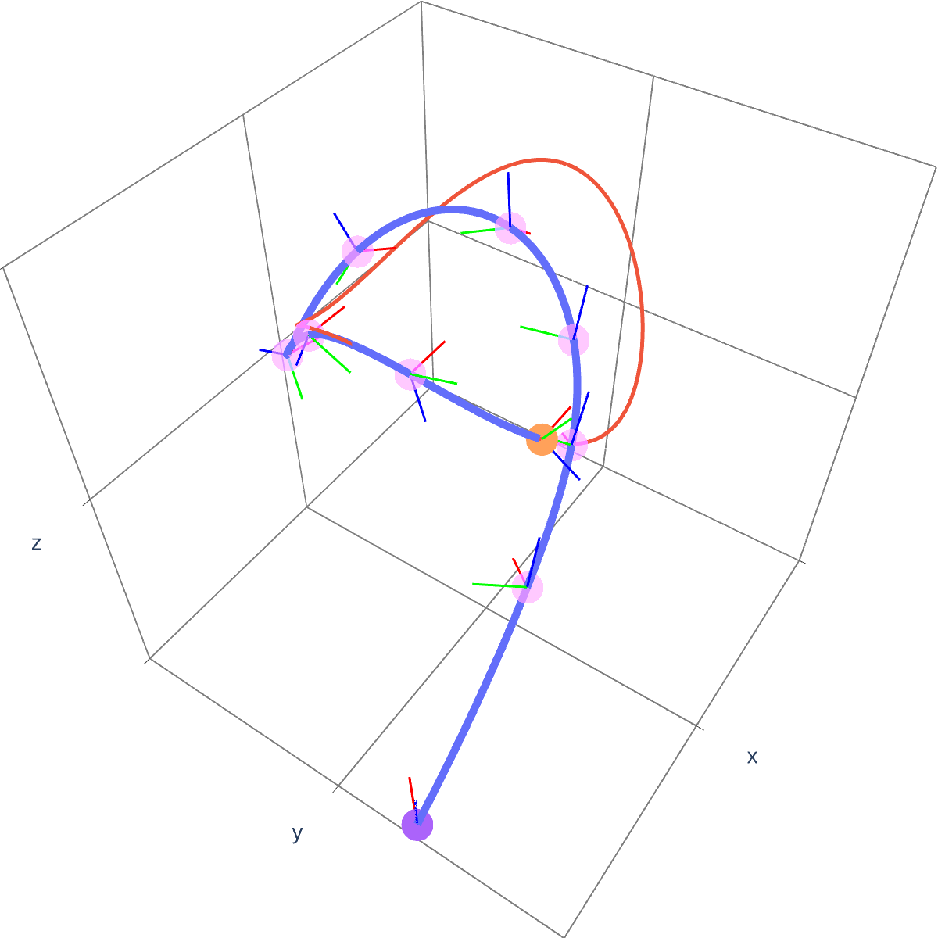
\includegraphics[width=\textwidth]{figures/vf_automatica_1.pdf} % Replace with your image
        \caption{$t\in[0, 5]s$}
        \label{fig:vfplot-first}
    \end{subfigure}
    \hfill
    % Second subfigure
    \begin{subfigure}[b]{0.32\textwidth}
        \centering
        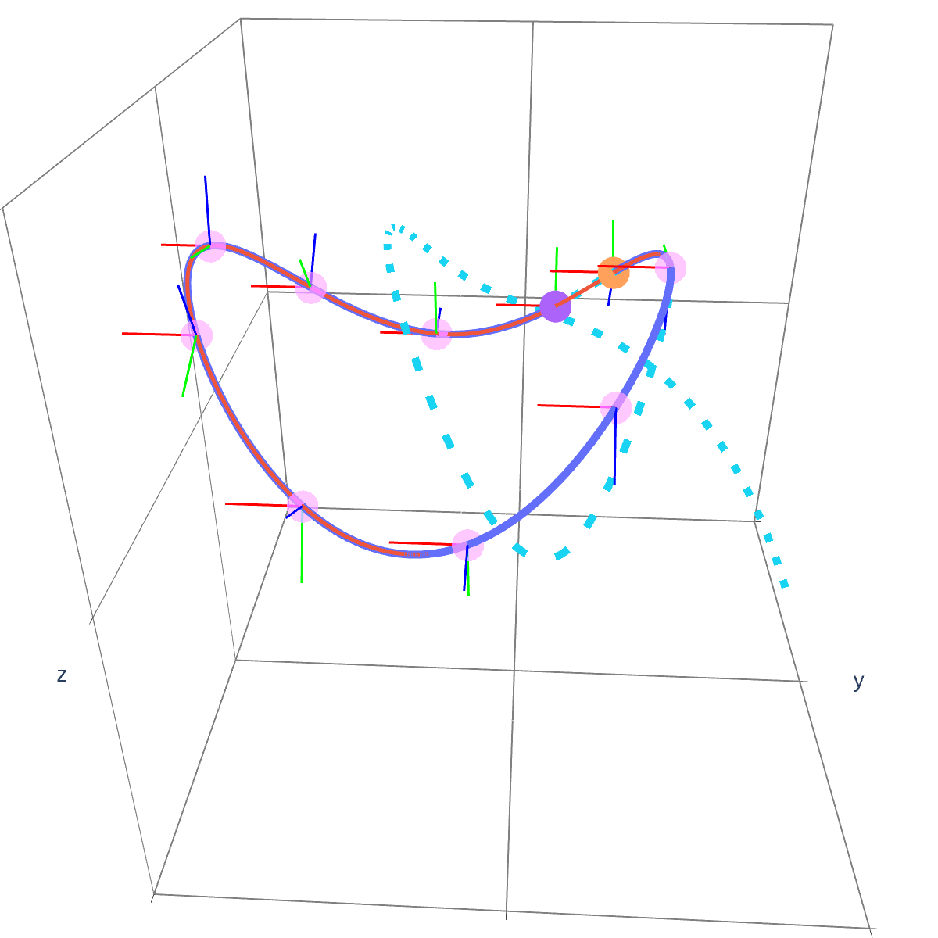
\includegraphics[width=\textwidth]{figures/vf_automatica_2.pdf} % Replace with your image
        \caption{$t\in[5, 9.7]s$}
        \label{fig:vfplot-second}
    \end{subfigure}
    \hfill
    % Third subfigure
    \begin{subfigure}[b]{0.32\textwidth}
        \centering
        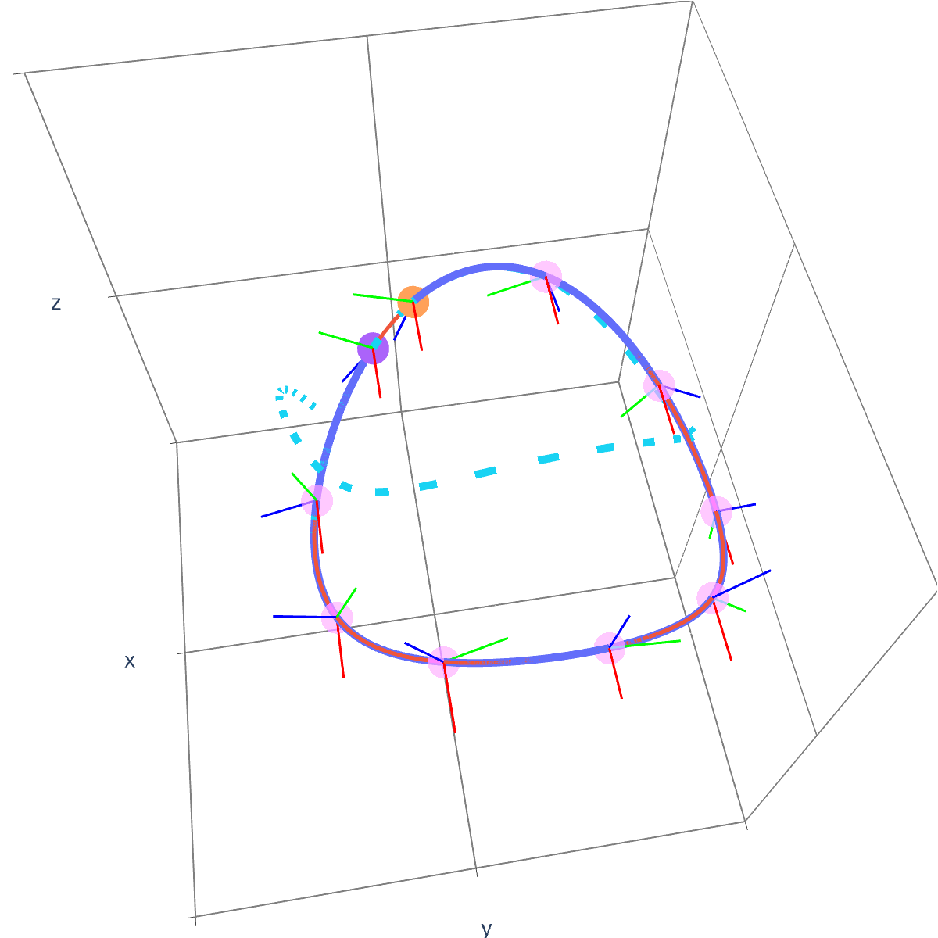
\includegraphics[width=\textwidth]{figures/vf_automatica_3.pdf} % Replace with your image
        \caption{$t\in[9.7, 14.5]s$}
        \label{fig:vfplot-third}
    \end{subfigure}
    \caption{The solid blue line depicts the system trajectory, while the solid red line indicates the target curve. The dashed light blue line represents the past trajectory. The initial and final positions are marked by purple and orange spheres, respectively. Translucent pink spheres denote intermediary positions, with orientation frames shown by RGB axes.}
    \label{fig:vfplot-trajectory}
\end{figure}
\begin{figure}[ht!]
    \centering
    \def\svgwidth{.8\linewidth}
    {\tiny\import{figures/}{distance_pos_ori_D.pdf_tex}}
    \caption{Value of EC-distance $D$, position error in centimeters and orientation error in degrees along time.}
    \label{fig:position-orientation-errors}
\end{figure}
We implemented the code in C++. On average, the computation of the vector field took $60\pm5$ milliseconds per iteration on a single core of an Intel i5-10300H @ 4.5GHz CPU, with 8 GB of RAM. On average, $99.5\%$ of this time was spent solving the optimization problem in \eqref{eq:optimization-problem-distance-definition-point-curve}. Since the optimization process is highly parallelizable -- allowing for the simultaneous computation of $\widehat{D}(\mathbf{H},\mathbf{H}_d(s))$ across different discretized $s$ -- the computational effort could be significantly reduced by leveraging parallel architectures such as GPUs, SIMD, or multi-threading. The system's trajectory is illustrated in \cref{fig:vfplot-trajectory}, while the values of the distance function $D$ are shown in \cref{fig:position-orientation-errors}. Additionally, \cref{fig:position-orientation-errors} provides a more intuitive representation of the position error (in centimeters) and the orientation error (in degrees). The results confirm that the system successfully converges to the desired curve and circulates around it as expected. Once the system reaches the curve, it remains there without deviation. Although our implementation was carried out in C++, we provide a less efficient sample code in Python for clarity and accessibility, available at \url{https://github.com/fbartelt/SE3-example/blob/main/SE3example.ipynb}.

\section{Collaborative Manipulation}
We conducted two simulations using UAIBot (\url{https://uaibot.github.io/}) to validate the theoretical results presented in this work. Firstly, we applied the vector field to a first-order integrator, followed by implementing the vector field-based adaptive control strategy. Both tasks focused on the convergence and circulation of a static curve in pose space.

In both simulations, we employed the forward Euler method with a time step of $\Delta t = \qty{1E-2}{\second}$. The parametric representation of the curve remained consistent across both simulations, with only minor variations in constants. Specifically, the parametric equation $\mathbf{h}(s)=(\mathbf{p}_d(s),\;\mathbf{R}_d(s))$ was defined as follows:
\begin{align}
\begin{split}
    \mathbf{p}_d(s) &= \begin{bmatrix}
        c_1(\sin(2\pi s) + 2\sin(4\pi s))\\
        c_1(\cos(2\pi s) - 2\cos(4\pi s))\\
        c_2 - c_1\sin(6\pi s)
    \end{bmatrix},\\
    \mathbf{R}_d(s) &= \mathbf{R}_z(2\pi s)\mathbf{R}_x(4\pi s),
    \end{split} \label{eq:parametriceq-simulation}
\end{align}
where $\mathbf{R}_z(a), \mathbf{R}_x(a)$ represent a rotation of $a$ radians around the $z$-axis and $x$-axis, respectively.

For the integration of rotation matrices, we utilized the exponential map \citep{Culbertson2021}:
\begin{equation}
    \mathbf{R}(t+\Delta t) \approx e^{\Delta t\SL[\boldsymbol{\omega}(t)]}\mathbf{R}(t). \label{eq:exponentialmap-integration-rotation}
\end{equation}
In practice, our curve parametrization was implemented as a list of tuples, with the $i$-th entry denoted as $\mathbf{h}[i]=(\mathbf{p}_d[i],\, \mathbf{R}_d[i])$. This allowed for an approximation of the tangent vector. Let $i^*$ represent the index of the curve that solves optimization problem \eqref{eq:otmproblemsStar}, then the tangent approximation was defined as
\begin{align}
    \mathbf{T} &\approx \begin{bmatrix}
        (\mathbf{p}_d[i^*\!\!+1] - \mathbf{p}_d[i^*])\slash\Delta s\\\vspace{1mm}
        \invSL[\ln\left(\mathbf{R}_d[i^*\!\!+1]\mathbf{R}_d^T[i^*]\right)]\slash\Delta s
    \end{bmatrix}, \label{eq:tangent-approximation}
\end{align}
with the angular component based on SLERP \citep[p. 104]{hanson2006visualizing}.

The time derivative of the vector field was also approximated using the following expression:
\begin{align}
    \dot{\boldsymbol{\psi}} \approx 
        \frac{\boldsymbol{\psi}\left(\mathbf{p}+\Delta t\dot{\mathbf{p}},\, \exp\left(\Delta t\SL[\boldsymbol{\omega}]\right)\mathbf{R}\right) - \boldsymbol{\psi}\left(\mathbf{p},\, \mathbf{R}\right)}{\Delta t}.
\end{align}
The functions $G$ and $H$ were defined as follows:
\begin{align}
    G = \frac{2}{\pi}\tan^{-1}\left(5\sqrt{D}\right),\quad
    H = \kappa\sqrt{1 - G^2}.
\end{align}
The parameter $\beta$ was set to $1$ for both simulations.

\subsection{Adaptive Dynamic}
\begin{table}[htb]
\begin{center}
\caption{Adaptive simulation parameters}\label{tb:parameters}\vspace{-2mm}
\begin{tabular}{clcl}
Parameter & Value & Parameter & Value\\\hline
$m$ & $\qty{1.28E3}{\kilogram}$ & $\mathbf{r}_{2}$ & $[0,\,0,\,-1.5]\,\unit{\meter}$\\
$I_\text{cm,xx}$ & $\qty{1.56E2}{\kilogram\meter\squared}$ & $\mathbf{r}_{3}$ & $[0.5,\,0,\,0]\,\unit{\meter}$\\
$I_\text{cm,yy}$ & $\qty{1.56E2}{\kilogram\meter\squared}$ & $\mathbf{r}_{4}$ & $[-0.5,\,0,\,0]\,\unit{\meter}$\\
$I_\text{cm,zz}$ & $\qty{4.93E1}{\kilogram\meter\squared}$ & $\mathbf{r}_{5}$ & $[0,\,0.5,\,0]\,\unit{\meter}$\\
$\mathbf{r}_{p}$ & $[0,\,0,\,1.5]\,\unit{\meter}$ & $\mathbf{r}_{6}$ & $[0,\,-0.5,\,0]\,\unit{\meter}$\\
$\mathbf{r}_{1}$ & $[0,\,0,\,1.5]\,\unit{\meter}$\\\hline
\end{tabular}
\end{center}
\end{table}
In this section, we investigate the manipulation of a large cylindrical body by six agents, aiming to converge to and circulate the curve parameterized by Eq. \eqref{eq:parametriceq-simulation}. The curve constants were set to $c_1 = 0.7$ and $c_2 = 0.4$, and $s$ was discretized into $5000$ evenly spaced samples within the interval $[0, 1]$, thus $\Delta s=1\slash5000$. For function $H$ we set $\kappa=1.4$. The cylindrical body had a radius of $\qty{0.25}{\meter}$ and a height of $\qty{1}{\meter}$, with additional parameters detailed in \cref{tb:parameters}. The agents were symmetrically distributed, and the measurement point was located at the position of the first agent. Additionally, the dead zone strategy \citep{ioannou2012robust} was employed for $\|\boldsymbol{\zeta}\| \le 0.01$, in which no adaptation will occur.

The adaptive parameters were set as $\boldsymbol{\Gamma}_r=\num{3E-4}\cdot\mathbf{I}_{3\times3},\, \boldsymbol{\Gamma}_o=\num{3E-2}\cdot\text{diag}(|\mathbf{o}_i| + \num{1E-2}) $, and $\mathbf{K}_D=1\slash6\cdot\text{diag}(\num{5E3}\cdot\mathbf{I}_{3\times3},\,\num{5E2}\cdot\mathbf{I}_{3\times3})$, where $\text{diag}(\cdot)$ maps a vector into a diagonal matrix or a list of matrices into a block diagonal matrix, and $|\cdot|$ is the element-wise absolute value. The object's initial position was set to $[-0.1,\, 0,\, 0.2]^T$, and the initial orientation was the identity matrix. The initial estimates $\hat{\mathbf{o}}_i$ and $\hat{\mathbf{r}}_i$ were randomly initialized with a normal distribution having zero mean and standard deviations of $1$ and $2$, respectively. The simulation duration was $\qty{20}{\second}$.
\begin{figure}[htb]
    \centering
    \includegraphics[width=.7\columnwidth]{figures/adaptive_errorNorm.pdf}
    \vspace{-1mm}
    \caption{Norm of error vector $\boldsymbol{\zeta}$ during the adaptive control simulation.}
    \label{fig:sim2-snorm}
\end{figure}
\begin{figure}[htb]
    \centering
    \includegraphics[width=.7\columnwidth]{figures/wrenches.pdf}
    \vspace{-1mm}
    \caption{Demmanded control inputs during the adaptive control simulation.}
    \label{fig:sim2-metricvalue}
\end{figure}

Throughout the adaptation process, the error vector $\boldsymbol{\zeta}$ exhibited oscillations, as depicted in \cref{fig:sim2-snorm}. However, it rapidly converged to zero after approximately $\qty{6.8}{\second}$. Analyzing \cref{fig:sim2-metricvalue}, it is evident that the object approached the curve asymptotically earlier, at around $\qty{4.6}{\second}$, indicating robust performance. Subsequently, after $\qty{6.8}{\second}$, the object closely followed the curve, which is expected when $\|\boldsymbol{\zeta}\|\approx0$, in line with our theoretical foundation.